\begin{frame}[t]{Background}

\begin{columns}
\begin{column}{0.6\textwidth}
    \begin{itemize}
        \item Nodes must be axially homogeneous
        \item Control rod positions often do not align with node boundaries, 
        requiring homogenization of control rod and moderator
        \item Volume homogenization preserves material volume/mass, but not 
        reaction rates
        \item Two approaches to prevent rod cusping:
        \begin{itemize}
          \item Refine mesh to align with all control rod positions
          \item Decusping method to improve homogenization
        \end{itemize}
    \end{itemize}
\end{column}
\begin{column}{0.4\textwidth}
\begin{figure}[h]
  \centering
  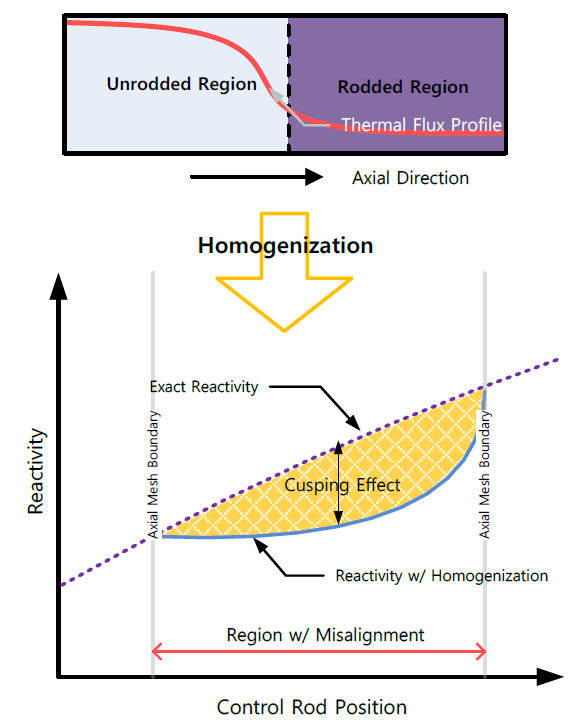
\includegraphics[width=\textwidth]{cusping_effect_Joo.png}
\end{figure} 
\end{column}
\end{columns}
    
\end{frame}

%%%%%%%%%%%%%%%%%%%%%%%%%%%%%%%%%%%%%%%%%%%%%%%%%%%%%%%%%%%%%%%%%%%%%%%%%%%%%%%%%

\begin{frame}[t]{2D/1D Decusping Methods}
    
    \begin{itemize}
        \item Neighbor Spectral Index Method - CRX-2K 
        \cite{cho2015CRX2d1dFusionDecusping}
        \begin{itemize}
          \item Spectral index is defined as the ratio of the fast flux to the 
          thermal flux
          \item Spectral index is used in top and bottom neighbor nodes to 
          estimate partially rodded node flux profile
          \item This estimate is used to update cross-sections 
          each iteration
        \end{itemize}
        \item nTRACER Method \cite{ICAPPcontrolRodDecuspingNTRACER}
        \begin{itemize}
          \item Solves local problem to generate CMFD constants
          \item Performs CMFD calculations on fine mesh to obtain axial flux 
          profiles
          \item Uses axial flux profiles during full core calculation to 
          homogenize cross-sections
        \end{itemize}
        \item Polynomial Decusping - MPACT \cite{MC2015_VCS_Cycle_Depletion}
        \begin{itemize}
          \item A series of 3x3 assembly cases were run with partially rodded 
          nodes in the center assembly
          \item Results were used to generate polynomials of decusping error as 
          function of rod insertion
          \item Polynomials are used to reduce the control rod volume fraction 
          when homogenizing
        \end{itemize}
    \end{itemize}
    
\end{frame}

%%%%%%%%%%%%%%%%%%%%%%%%%%%%%%%%%%%%%%%%%%%%%%%%%%%%%%%%%%%%%%%%%%%%%%%%%%%%%%%%%

\begin{frame}[t]{Sub-Plane Decusping}
    
\begin{itemize}
    \item Modifications made to sub-plane scheme\footnote{Two M{\&}C 2017 papers submitted on sub-plane and decusping methods \cite{Graham2017Improvementofthe2D/1DMethodUsingtheSub-PlaneScheme,Graham2017RodDecuspingTechniquesforthe2D/1DMethod}} to treat axial effects of rod 
    cusping
    \begin{itemize}
      \item Homogenization still uses MOC flux with axial shape factor, but 
      with heterogeneous rodded or unrodded cross-sections
      \item Projection re-homogenizes cross-sections in partially rodded nodes 
      after CMFD calculation
    \end{itemize}
    \begin{equation}\label{e:nTRACERdecusping}
    \overline{\Sigma_i} = \frac{\phi_{rad,i}^R \phi_{ax,i}^R \Sigma_i^R h^R + \phi_{rad,i}^U \phi_{ax,i}^U \Sigma_i^U h^U}{\phi_{rad,i}^R \phi_{ax,i}^R h^R + \phi_{rad,i}^U \phi_{ax,i}^U h^U} \nonumber
    \end{equation}
\end{itemize}
    
\end{frame}

%%%%%%%%%%%%%%%%%%%%%%%%%%%%%%%%%%%%%%%%%%%%%%%%%%%%%%%%%%%%%%%%%%%%%%%%%%%%%%%%%

\begin{frame}[t]{Collision Probabilities Decusping}
    
\begin{columns}
    \begin{column}{0.45\textwidth}
      \begin{itemize}
        \item Sub-plane modifications only capture axial effects
        \begin{itemize}
          \item MOC uses homogenized cross-section
          \item Radial shape does not accurately reflect either region
        \end{itemize}
        \item 1D collision probabilities (CP) introduced to generate radial 
        shapes
        \begin{itemize}
          \item Generates radial flux profile for rodded and unrodded region
          \item Radial profiles used in CMFD homogenization
          \item Very efficient calculation
        \end{itemize}
      \end{itemize}
    \end{column}
    \begin{column}{0.55\textwidth}
    \begin{figure}[h]
      \centering
      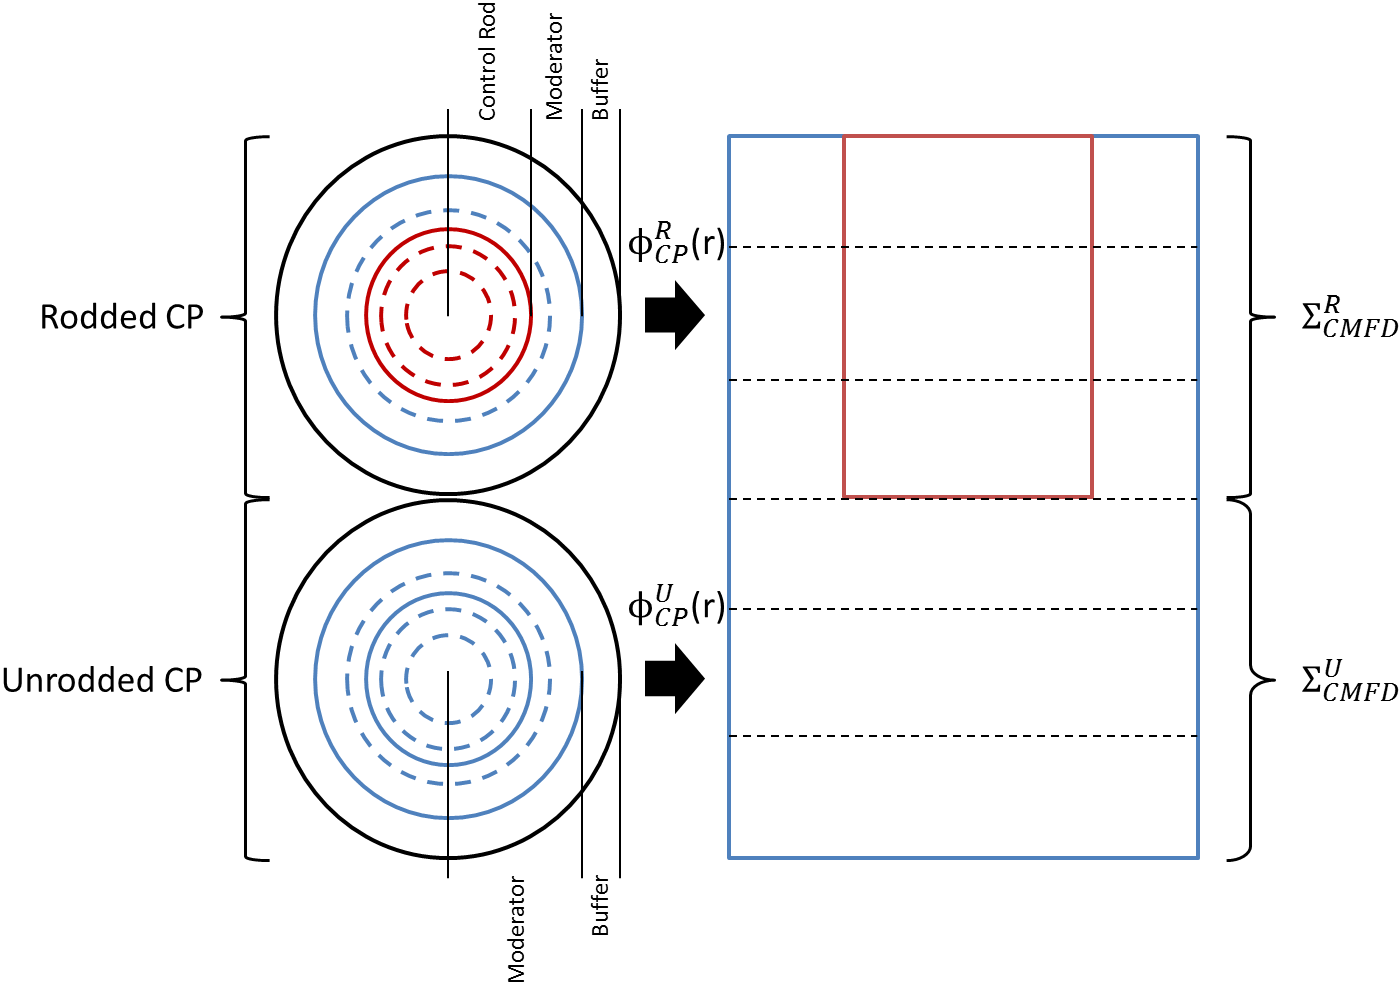
\includegraphics[width=\textwidth]{CPdecusp.png}
    \end{figure}
\end{column}
\end{columns}
    
\end{frame}